\begin{figure}
 \caption{Network Topology Diagram}
  \centering
   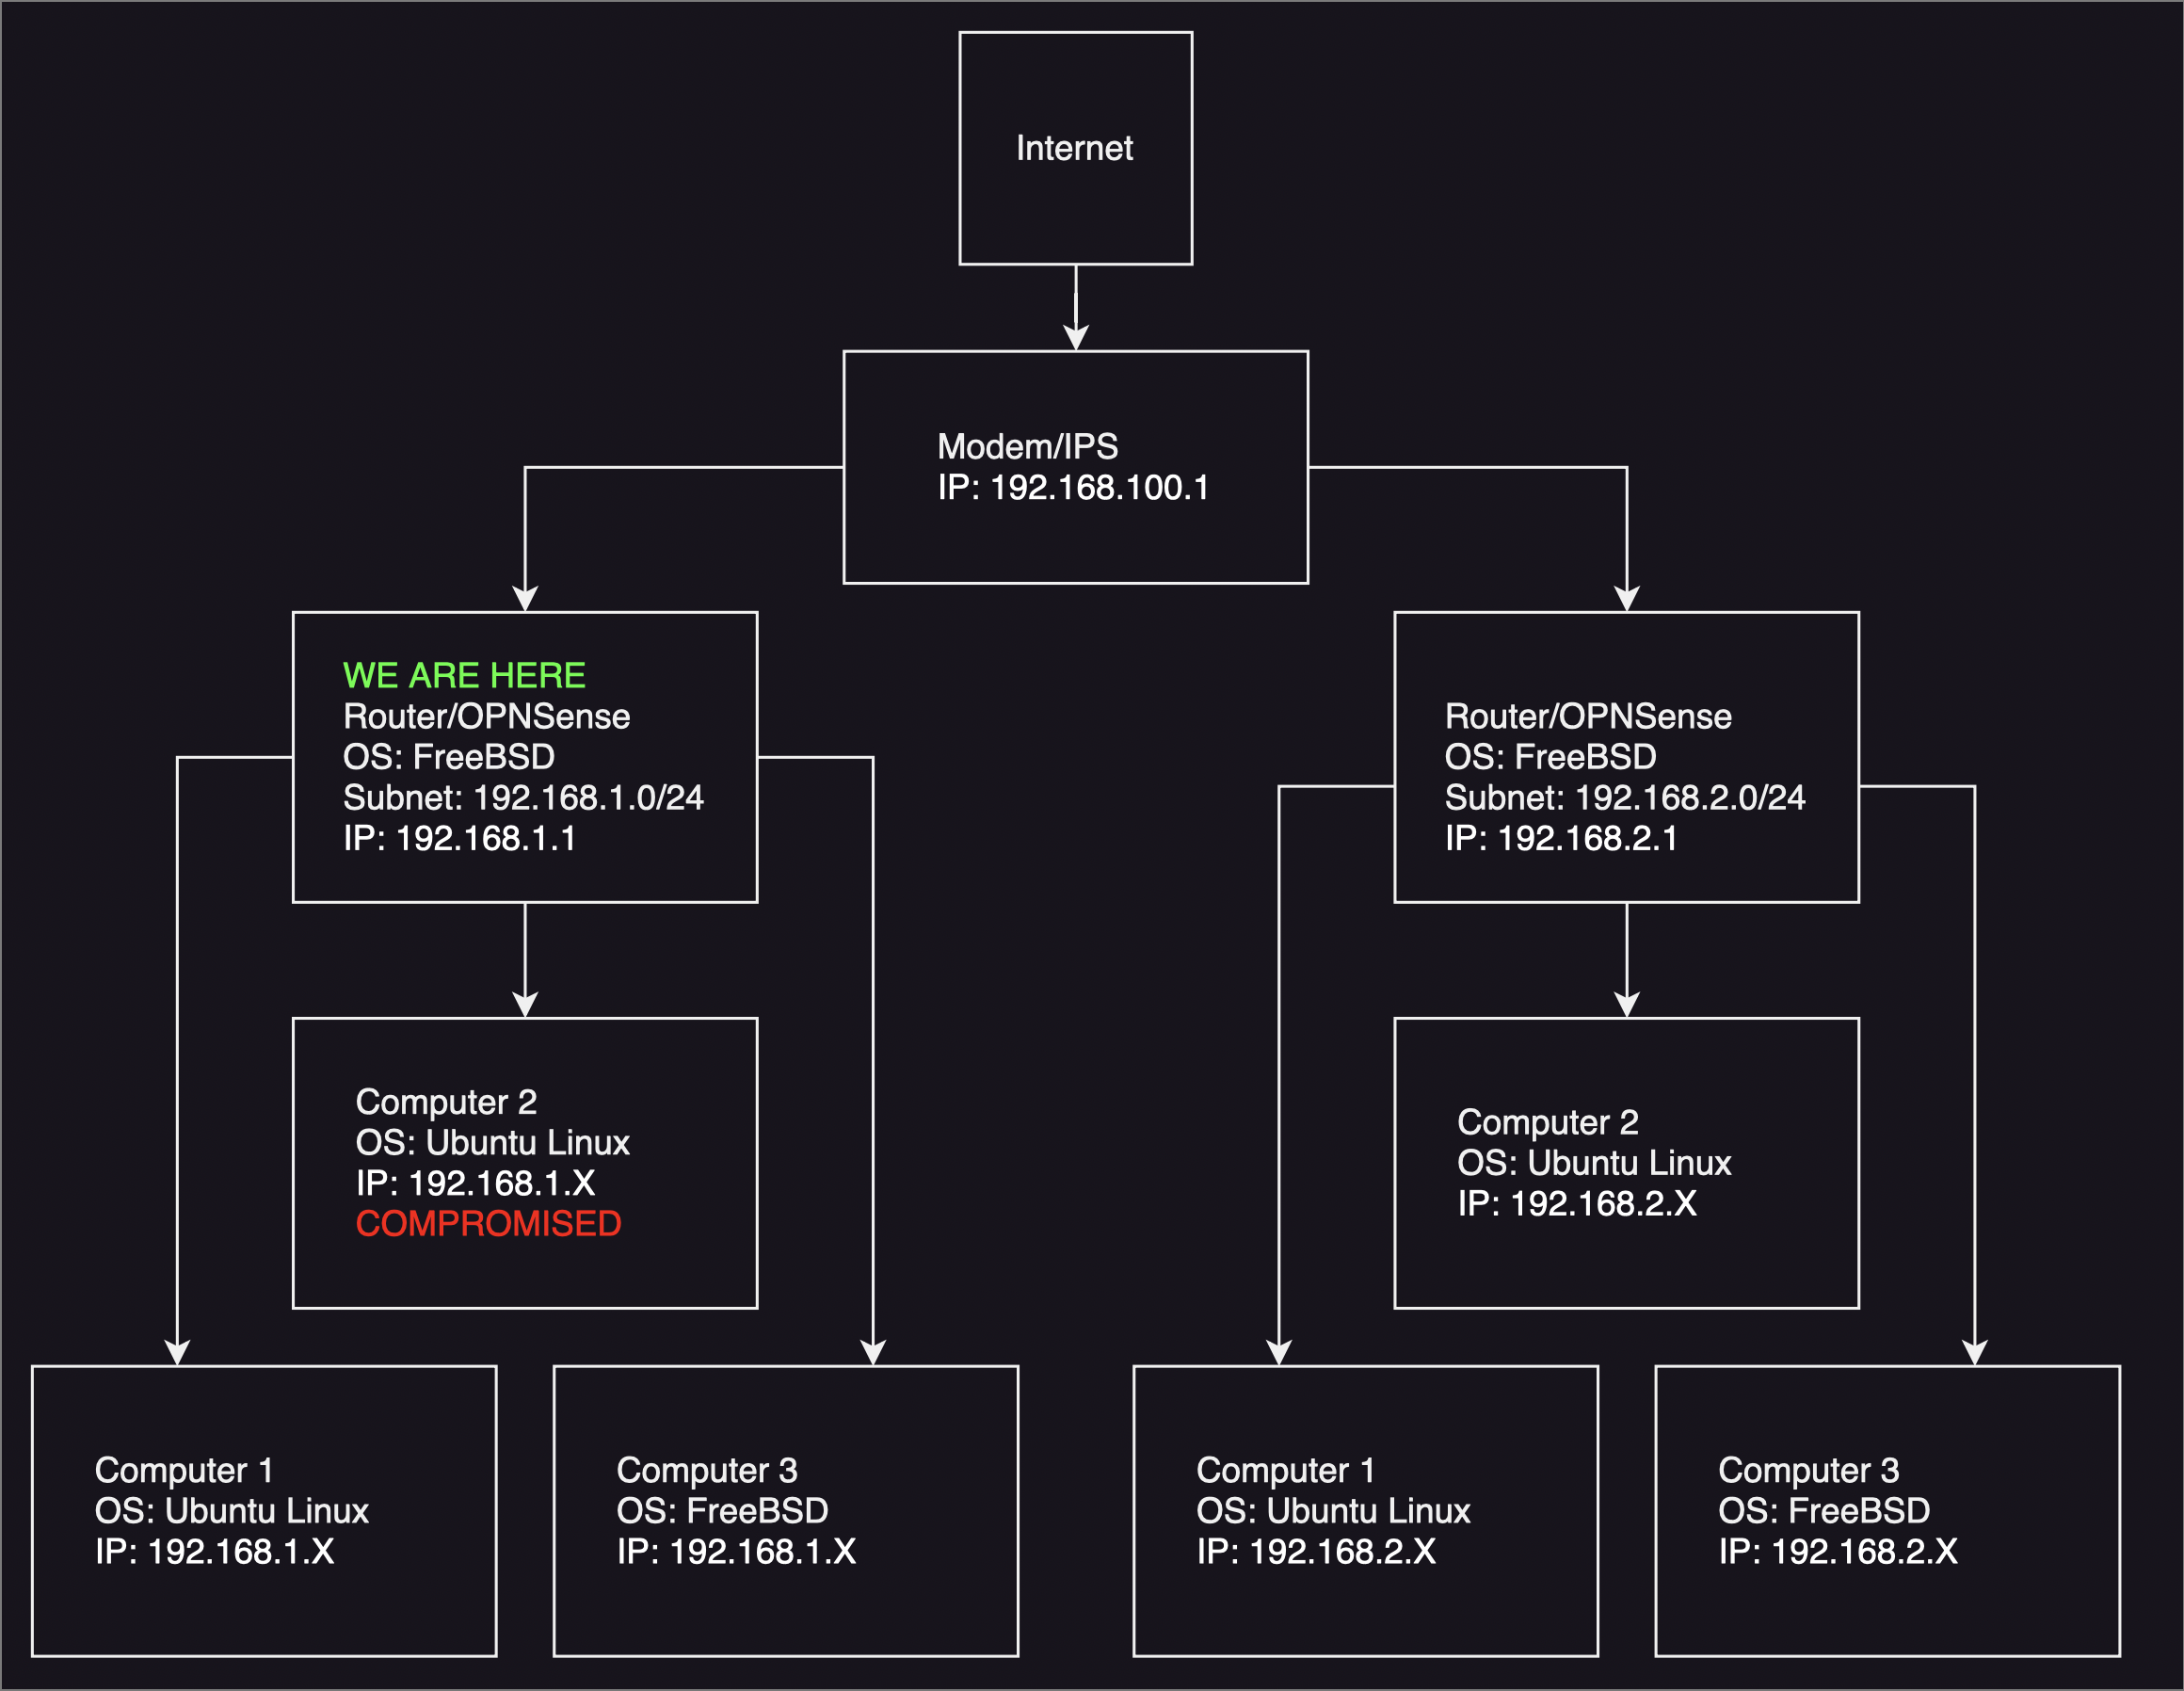
\includegraphics[width=0.5\textwidth]{diagram.png}
   \label{fig:network-topology}
\end{figure}

%-------------------------------------------------------------------------------

Our threat model concerns the scenario in which a system is attacked. Specifically, we focus on the scenario depicted in Figure~\ref{fig:network-topology}, where three interconnected computers form a subnet, with one of these computers compromised. Within this context, our threat model revolves around an attacker who has successfully gained access to one of the systems, as illustrated in the diagram. Once inside the network, the attacker's assumed objective is to scan other systems to identify vulnerabilities for lateral movement. The provided script, named ip-shuffle, plays a crucial role in this threat model, as it allows for the dynamic assignment of random IP addresses to network interfaces. The attackers' assumed capabilities are that they have basic user access to the compromised system, can perform network reconnaissance via scanning the network, and system persistence. 
